\documentclass[10pt,twocolumn,letterpaper]{article}
\usepackage{array}
\usepackage{statcourse}
\usepackage{times}
\usepackage{epsfig}
\usepackage{graphicx}
\usepackage{amsmath}
\usepackage{amssymb}
\usepackage{booktabs}
\usepackage{multirow}
\usepackage{hyperref}
\usepackage{caption}
% Include other packages here, before hyperref.

% If you comment hyperref and then uncomment it, you should delete
% egpaper.aux before re-running latex.  (Or just hit 'q' on the first latex
% run, let it finish, and you should be clear).

\statcoursefinalcopy%

\setcounter{page}{1}
\begin{document}


%%%%%%%%%%%%%%%%%%%%%%%%%%%%%%%%%%%%%%%%%%%%%%%%%%%%%%%%%%%%%%%
% DO NOT EDIT ANYTHING ABOVE THIS LINE
% EXCEPT IF YOU LIKE TO USE ADDITIONAL PACKAGES
%%%%%%%%%%%%%%%%%%%%%%%%%%%%%%%%%%%%%%%%%%%%%%%%%%%%%%%%%%%%%%%



%%%%%%%%% TITLE
\title{Comparative Analysis of Machine Learning Models: \\Alexnet, VGG, Resnet, YOLO}

\author{Pham Duc An\\
{\tt\small 10422002}
\and
Tran Hai Duong\\
{\tt\small 10422021}
\and
Vo Thi Hong Ha\\
{\tt\small 10421015}
\and
Nguyen Hoang Anh Khoa\\
{\tt\small 10422037}
\and
Truong Hao Nhien\\
{\tt\small 10422062}
\and
Nguyen Song Thien Phuc\\
{\tt\small 10422067}\\
\\
\{\tt @student.vgu.edu.vn\}
\and
Bui Duc Xuan\\
{\tt\small 10422085}
}

\maketitle
%\thispagestyle{empty}



% MAIN ARTICLE GOES BELOW
%%%%%%%%%%%%%%%%%%%%%%%%%%%%%%%%%%%%%%%%%%%%%%%%%%%%%%%%%%%%%%%


%%%%%%%%% ABSTRACT
\begin{abstract}
   In this project, we conducted a comprehensive comparative analysis of prominent machine learning models, namely Alexnet, VGG, Resnet, and YOLO, with a focus on their efficacy in image recognition. Leveraging a curated dataset representative of diverse real-world scenarios with CIFAR-10, our study delved into the nuances of each model's architecture, training process, and computational requirements. Through rigorous evaluation using metrics such as accuracy, precision, and recall, our results reveal nuanced performance distinctions. Notably, Resnet demonstrated superior accuracy, VGG excelled in feature extraction, YOLO showcased real-time efficiency, and Alexnet exhibited a stable performance. These findings provide valuable insights for practitioners and researchers seeking to optimize model selection for specific applications, shedding light on the trade-offs between accuracy, computational cost, and real-time processing capabilities. Project's detailed code are provided at {\url{https://github.com/nhientruong04/LIA-introCS-proj}}.
\end{abstract}

%%%%%%%%% BODY TEXT
\section{Experiments}
\subsection{Dataset}
This study leverages the CIFAR-10 dataset for training and evaluation. CIFAR-10 consists of 60,000 $32\times32$ color images in 10 different classes, with 6,000 images per class. This dataset is widely used for image classification tasks, providing a diverse set of small-sized images for training robust models.

\subsection{Settings}
Typically, conducting a thorough experiment would be redundant since training and testing with each combination of hyperparameters would cost us a lot of time and resources. Therefore, we conducted an experiment which required a fixed setting and guaranteed homogeneity for all targeted models. The set of hyperparameters are configured in Tab \ref{tab:settings}.

\begin{table}
        \begin{center}
            \begin{tabular}{c|c}
                \hline
                \textbf{Settings} & \textbf{Value} \\
                \hline
                        Learning rate & 0.01\\
                        Epoch & 20 \\
                        Batch size & 64 - 128 \\
                        Input size & (224 x 224) \\
                        Augmentation & Random flip, RGB normalization \\
                        Dataset splits & Train-val-test (0.8-0.1-0.1) \\
                \hline
            \end{tabular}
            \caption{Settings for training and final comparison.}
            \label{tab:settings}
        \end{center}
\end{table}

It is not quite common to set the learning rate at $1e-2$ as it is considered unnecessary large, a more common learning rate is $1e-3$. However, for the sake of convergence speed of the chosen models, we chose this rate and adopted a “Reduce Learning Rate on Plateau” scheduler \cite{reduceonplateau} to have better results. Regarding the optimizer algorithm, Stochastic Gradient Descent \cite{SGD} was used because of its popularity and widely approved efficiency, with a weight decay of $0.01$ and $0.9$ momentum. Both training and testing procedures are conducted on a T4 GPU (with 15 GB VRam) provided by Google Colab and a local NVIDIA RTX 2060 (with 12 GB VRam).

\subsection{Result}
After 20 epochs of training, important metrics such as precision, recall and accuracy were logged\footnote[3]{YOLO metrics were not included. Please visit its official implemented pipeline at \url{https://github.com/ultralytics/ultralytics} for information of its metrics and training settings.}. Recorded values can be viewed in Fig \ref{fig:precision} and Fig \ref{fig:recall}.
\begin{figure}
        \begin{center}
            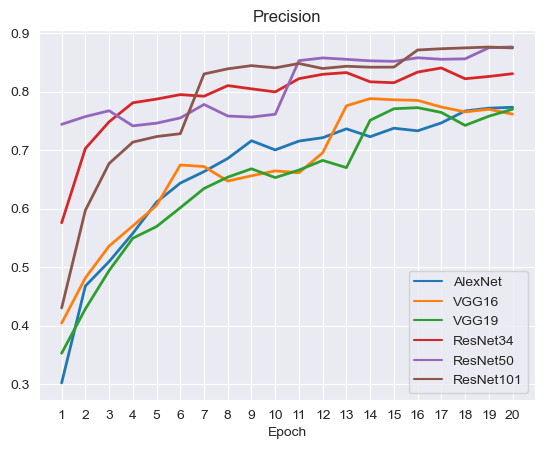
\includegraphics[width=0.45\textwidth]{figures/precision.png}
            \caption{Precision of all models on validation split. ResNet-50 and ResNet-101 both achieved the highest score.}
            \label{fig:precision}
        \end{center}
\end{figure}
\begin{figure}
        \begin{center}
            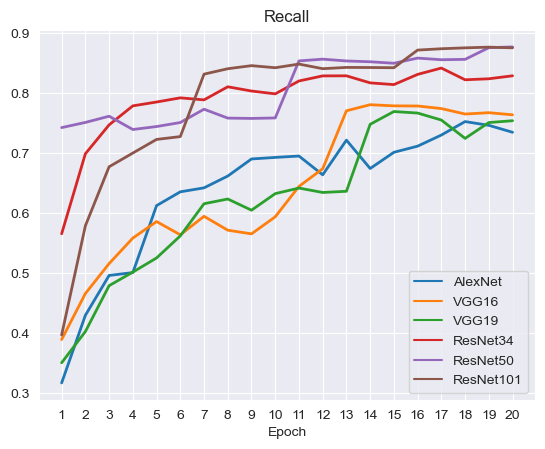
\includegraphics[width=0.45\textwidth]{figures/recall.png}
            \caption{Recall of all models on validation split. ResNet-50 and ResNet-101 both achieved the highest score.}
            \label{fig:recall}
        \end{center}
\end{figure}

The results of all tested models on the valuation set can be logically reasoned. These metrics indicate that a newer architecture would result in a better performance, since each model was proposed based on the fact that it has achieved or even surpassed the SOTA result at that time. AlexNet is the oldest model that has been proposed; hence, it performed generally worse compared to other models despite its unarguably good performance when compared to older Machine Learning techniques that mainly rely on feature extraction methods with mathematics. However, it is clear that these graphs reflect a quite opposite trend that we expected, which is the instability and fluctuation of the 2 VGG variants. At some points, including the $20^{th}$ epoch, both metrics of these 2 versions are lower than those of AlexNet. This strange phenomenon contradicts the common sense that we have introduced - the more parameters a model has, the more complex it is, the better it performs. Compared to AlexNet, VGGNet is far more complicated with a double amount of parameters that AlexNet has; which should imply that its variants would have better results. Regarding this peculiar problem, we propose a hypothesis for reasoning. We believe that each model has its own convergence timeline; which means that although both variants in this study perform worse than AlexNet, they should achieve better results when they are trained for longer time. Generally, 20 epochs are widely considered insufficient in order to evaluate the best result that a model can achieve; hence, training for sufficiently larger amount of epochs would result in a more logical output. 

Besides results logged after each epoch, an evaluation on the test set with $10,000$ images are also provided below.

\begin{table}[h]
        \centering
        \label{tab:small_table}
        \scalebox{1}{\begin{tabular}{c|c|c|c}
        \hline
        
        \textbf{Model} & \textbf{Accuracy} & \textbf{Precision} & \textbf{Recall} \\
        \hline
                AlexNet & 0.755 & 0.7726 & 0.755 \\
                VGG-16 & 0.7781 & 0.7773 & 0.7781 \\
                ResNet-34 & 0.8431 & 0.8424 & 0.8431 \\
                ResNet-50 & 0.8653 & 0.8657 & 0.8653 \\
                ResNet101 & \underline{0.8848} & \underline{0.8851} & \underline{0.8848} \\
                Yolov8n-cls & \textbf{0.8896} & \textbf{0.8892} & \textbf{0.8896} \\
        \hline
        \end{tabular}}
        \caption{Result on test set. \textbf{Bold} values are largest, \underline{underline} values are second largest}
\end{table}

YOLOv8 nano with classification version achieved the best result, which is slightly better than the ResNet-101. YOLO is a complicated pipeline with different modules and parts that are regressed to produce the final result; hence its dominant result is understandable. In fact, considering only plain models would make ResNet stand out the most with its high performance in all of its 3 versions. This is also the reason why ResNet is widely utilized as a firm backbone for various pipelines and recent architectures.

{\small
        \bibliographystyle{ieee}
        \bibliography{bibliography.bib}
}


\end{document}